% Standard LaTeX document template
%  BE SURE TO PROCESS DOCUMENT TWICE IF IT CONTAINS CROSS-REFERENCES!

\documentclass[12pt]{article}
\usepackage[round]{natbib} %allow to set the bibliography style and
% import the bibliography file. See Bibliography management with
% natbib for more information on
% https://www.sharelatex.com/learn/Bibliography_management_with_natbib.
% See the reference sheet for natbib on
% http://merkel.zoneo.net/Latex/natbib.php.
% Several .bst files can be
% downloaded from http://kinglab.eeb.lsa.umich.edu/pub/biblios/bst/

\usepackage{graphicx,epsfig}
\usepackage{amssymb,amsmath,amsfonts,bm,color,supertabular,longtable,multirow}
\usepackage[colorlinks=true,linkcolor=black,citecolor=black,urlcolor=black]{hyperref}

\setlength{\oddsidemargin}{0in} % left margin, odd pages
\setlength{\evensidemargin}{0in} % left margin, even pages
\setlength{\textwidth}{6.5in} % widtth of text on page
\setlength{\topmargin}{-.3in} % add to default 1 in
\setlength{\headsep}{0in}     % add to default 25pt
\setlength{\textheight}{8.7in}  % height of text on page
\setlength{\parskip}{.1in}            % vertical space between paragraphs
\setcounter{tocdepth}{2}

%\setlength{\parindent}{0in}            % amount of indentation of paragraph


%  newcommands -- more newcommands used in the document.
%  not just in the preamble

\newcommand{\Var}{\mbox{Var}}
\newcommand{\Cov}{\mbox{Cov}}
\newcommand{\E}{\mbox{E}}
\newcommand{\ubeta}{\mbox{\boldmath$\beta$}}
% Independence symbol
\newcommand\independent{\protect\mathpalette{\protect\independenT}{\perp}}
\def\independenT#1#2{\mathrel{\rlap{$#1#2$}\mkern2mu{#1#2}}}


\title{STAT 501 Case Study Assignment} 
\author{Quan Zhao\\
School of Mathematics and Statistics\\ Victoria University of Wellington, New Zealand} 
%\date{}  % Add \date{} to make a blank date.


%  main body of document

\begin{document}

% Titlepage
\maketitle

\begin{abstract}
  This course provides students with an opportunity to develop their
  research skills in Mathematics and Statistics, including use of
  library resources, constructing literature reviews, developing
  research questions, writing research proposals, and developing
  skills in oral presentation. The template file gives an introduction
  to LaTeX,
\end{abstract}


% Table of Contents
\tableofcontents


\setlength{\baselineskip}{0.25in} % min space from bottom of one line

                                 % to top of next in a paragraph

                                 % place after \begin{document}



\newpage  % start from a new page
\section{Introduction}

\label{s.intro}

The relationship between students' interest and aptitude in science and the overall development of countries on a global scale is a subject that is both fascinating and deserving of in-depth analysis. Understanding this relationship can offer valuable insights into the educational, economic, and social fabric of nations.

In this comprehensive study, we aim to shed light on this complex issue by conducting a rigorous statistical analysis at the national level. To achieve this, we have integrated multiple data sources, including the Programme for International Student Assessment (PISA) and the Human Development Index (HDI) from United Nations data. PISA provides a robust measure of 15-year-old students' science literacy, while the HDI offers a composite index of life expectancy, education, and per capita income indicators, which are used to rank countries into tiers of human development.

Our primary objective is to offer a high-level overview that elucidates the relationship between students' scientific capabilities and interests and their country's level of development. By doing so, we aim to identify key issues that may be hindering progress in both educational and developmental sectors. Furthermore, our analysis serves as a foundation for proposing actionable solutions that could be implemented to improve educational outcomes and, by extension, the overall well-being of nations.

Through this study, we hope to contribute to the ongoing discourse on education and development, providing policymakers, educators, and stakeholders with valuable data and insights that can guide future initiatives and reforms.

% Context and background information.
% \cite{Liu05}

% \section{Objectives and Scope}

% %Specific objectives of the statistical consultation.
% %Scope of the analysis including what is and is not covered.

% \begin{itemize}
%   \item Identify the top ten countries in overall sciences scores.
%   \item Determine whether wealthier (higher income) countries tend to provide more support.
%   \item Determine whether students from countries with a higher HDI show more interest in science.
%   \item Determine whether the level of support and interest have an effect on overall science scores.
% \end{itemize}

\section{Objectives and Scope}

\label{s.objectives}

This study aims to provide a comprehensive understanding of the relationship between students' interest and aptitude in science and the overall development of their respective countries. To achieve this, we have outlined the following specific objectives:

\begin{itemize}
\item \textbf{Science Literacy Rankings:} Identify the top ten countries with the highest overall science scores based on PISA assessments. This will serve as a benchmark for evaluating the effectiveness of educational systems in fostering scientific literacy.

\item \textbf{Wealth and Educational Support:} Investigate whether countries with higher per capita income levels tend to provide more educational support in science. Support could be measured in terms of educational funding, availability of science programs, and teacher-to-student ratios.

\item \textbf{Human Development and Scientific Interest:} Examine the correlation between a country's Human Development Index (HDI) and the level of interest in science among its students. Interest could be gauged through survey data, extracurricular participation, or other relevant metrics.

\item \textbf{Impact of Support and Interest:} Assess whether the level of educational support and student interest in science have a significant impact on overall science scores. This will involve multivariate statistical analyses to control for other influencing factors.
\end{itemize}

\textbf{Scope of Analysis:}

The scope of this study is limited to:

\begin{itemize}
\item Data from the most recent PISA assessments, focusing on 15-year-old students' performance in science.

\item HDI data from the United Nations, specifically examining the components related to education and income.

\item Countries for which both PISA and HDI data are available, to ensure a comprehensive and comparative analysis.
\end{itemize}

This study will not cover:

\begin{itemize}
\item In-depth analyses of individual educational systems or curricula.

\item Factors such as cultural attitudes or government policies, unless they are directly related to educational support or student interest in science.
\end{itemize}

By adhering to these objectives and scope, we aim to provide a robust analysis that can inform policy decisions and educational reforms aimed at improving both educational outcomes and national development.

% \section{Methodology}

% Overview of the statistical methods used.
% Software and tools used for analysis.

\section{Data Description}

% # Sources of data.
% # Description of variables.
% # Data collection methods.
% # Data quality and validation procedures.

\subsection{Programme for International Student Assessment (PISA)}

\label{ss.pisa}
PISA is the OECD's Programme for International Student Assessment. PISA measures 15-year-olds’ ability to use their reading, mathematics and science knowledge and skills to meet real-life challenges.

We involved, Overall Science Score (average score for 15 year olds),  Interest in science, Support for scientific inquiry, etc. 

\subsection{Human Development Index (HDI)}

\label{ss.hdi}
Human Development Index (HDI)The HDI is a summary measure for assessing long-term progress in three basic dimensions of human development: a long and healthy life, access to knowledge and a decent standard of living.

In this work, we involved Income Index, Health Index, Education Index and Overall Human Development Index.

\section{Preliminary Data Analysis}

% Descriptive statistics.
% Data visualization.
% Identification of outliers or anomalies.

This Dataset has 64 country level summarise data.


\subsection{Data Imputation}
\label{ss.imputation}

In Figure $\ref{fig:missing}$ (a) shows the missing data info in raw data.
As PISA and HDI do not have correlation relationship, 
thus we do not keep rows which all PISA info or all HDI info missed.

In Figure $\ref{fig:missing}$ (b) shows the missing info after filter.
There are 54 country level observisons left.

We replace missing values by R MICE "predictive mean matching" (PMM) approach.


\label{ss.imputataion}

\begin{figure}[htb]
  \begin{minipage}[b]{1.0\linewidth}
    \centering
    \centerline{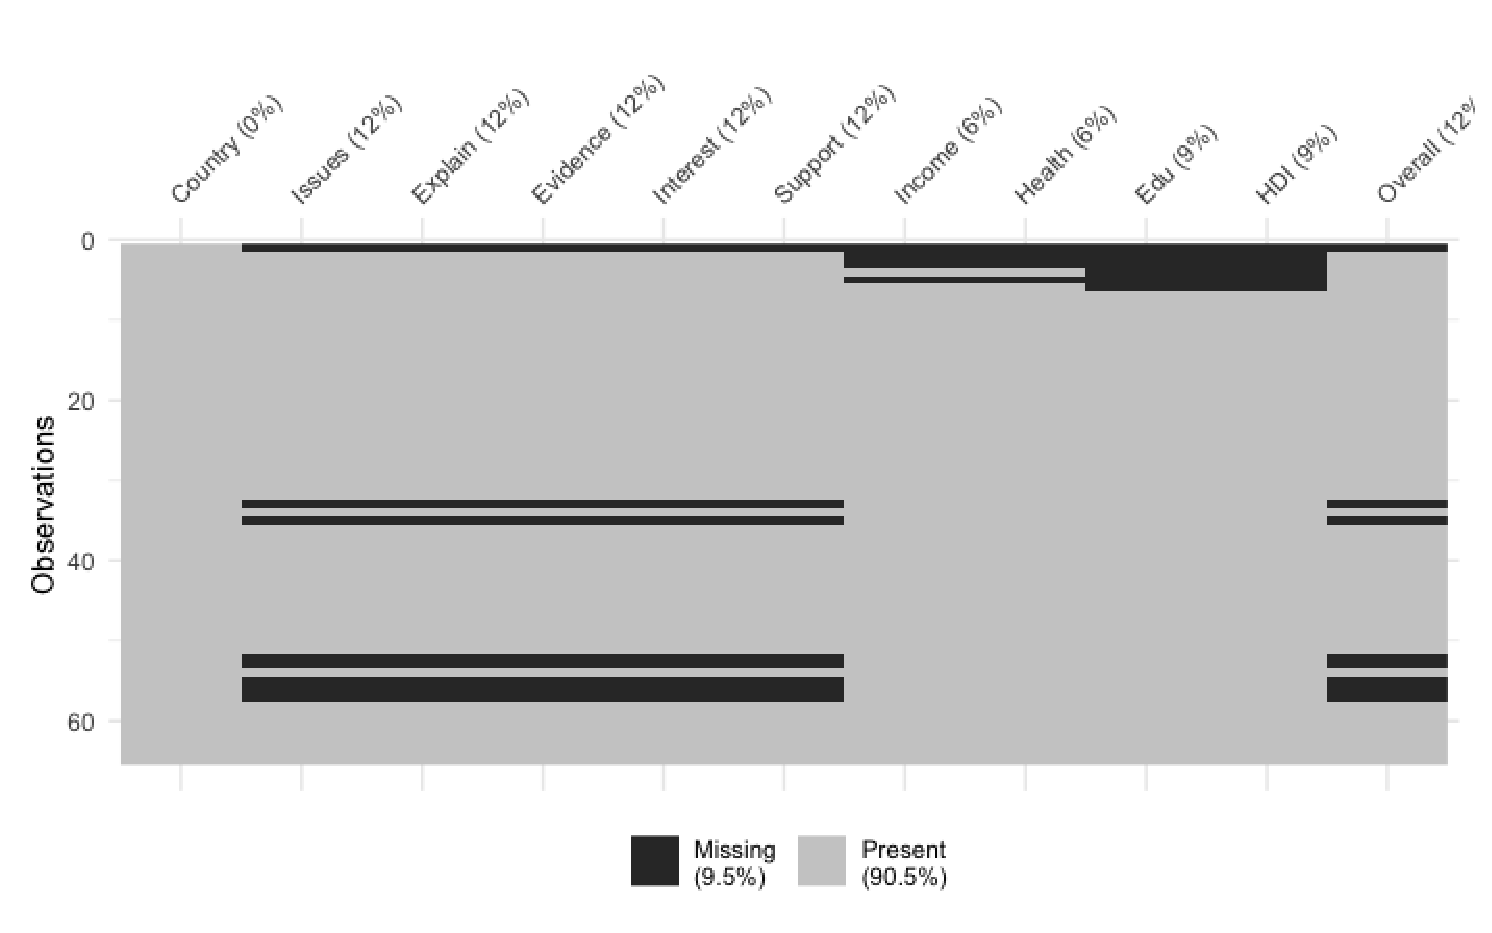
\includegraphics[width=7.0cm]{images/null_1}}
  %  \vspace{1.5cm}
    \centerline{(a) raw data}\medskip
  \end{minipage}
  \hfill
  \begin{minipage}[b]{1.0\linewidth}
    \centering
    \centerline{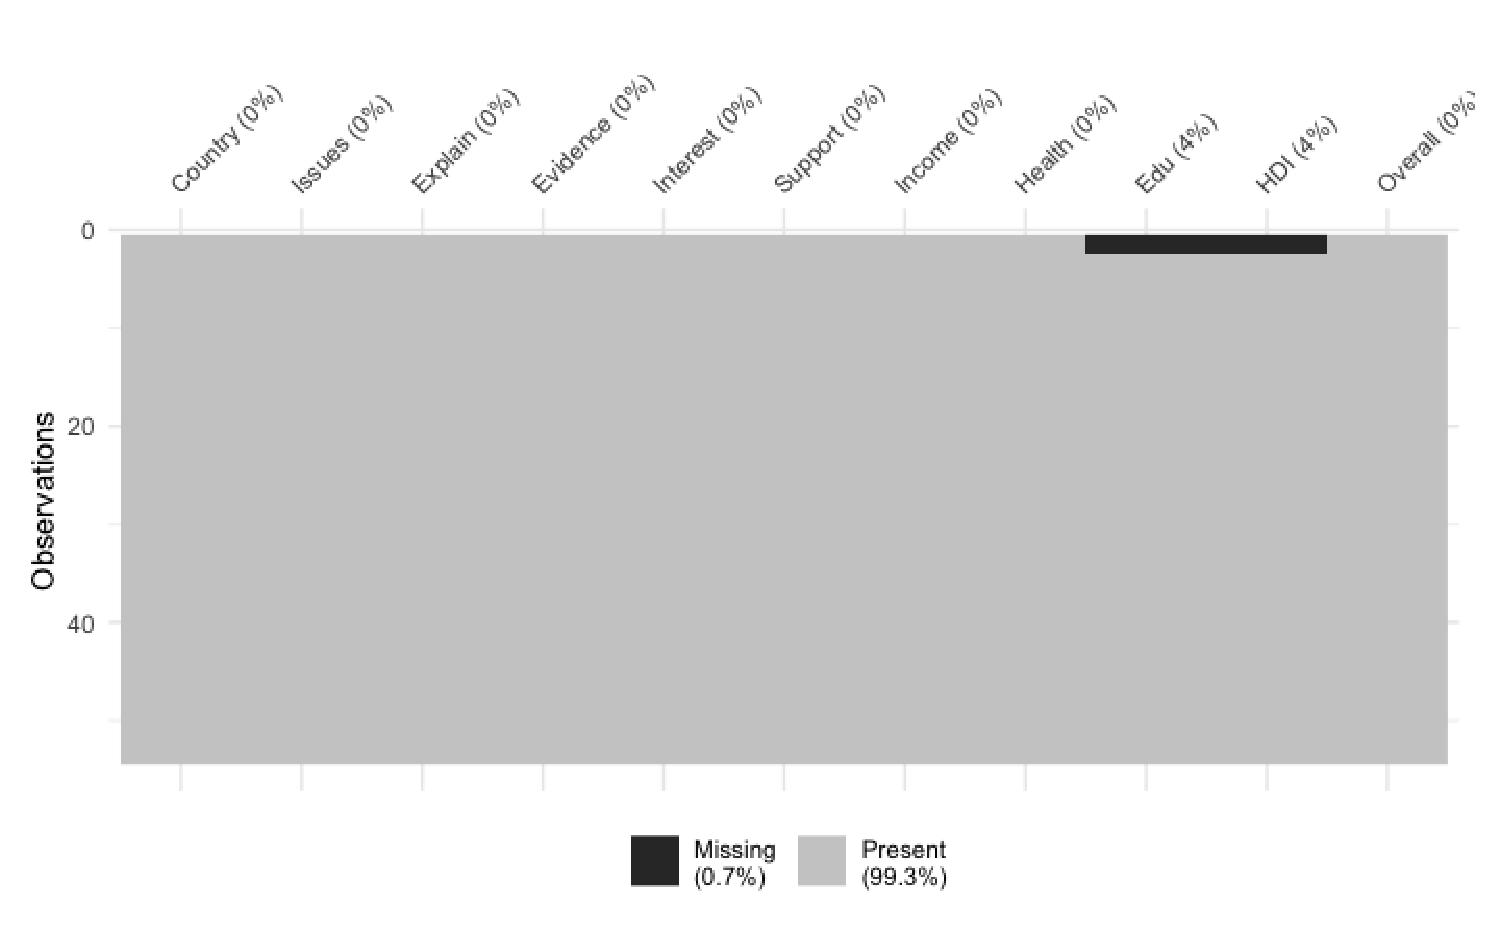
\includegraphics[width=7.0cm]{images/null_2}}
  %  \vspace{1.5cm}
    \centerline{(b) remove missing }\medskip
  \end{minipage}
  %
  \caption{Visualize Missing Data}
  \label{fig:missing}
  %
  \end{figure}


\section{Statistical Models and Techniques Used}
% Statistical tests conducted.
% Models fitted to the data.
% Model validation techniques.

\subsection{Correlation Analysis}
\label{ss.corr}

In Fig $\ref{fig:corr}$ shows all variable in linear correlation.
Income shows negative correlation to Support,
HDI shows negative correlation to interest,
and both Support and interest shows negative collection to Overall Score.


\begin{figure}[htb]
  \centering
  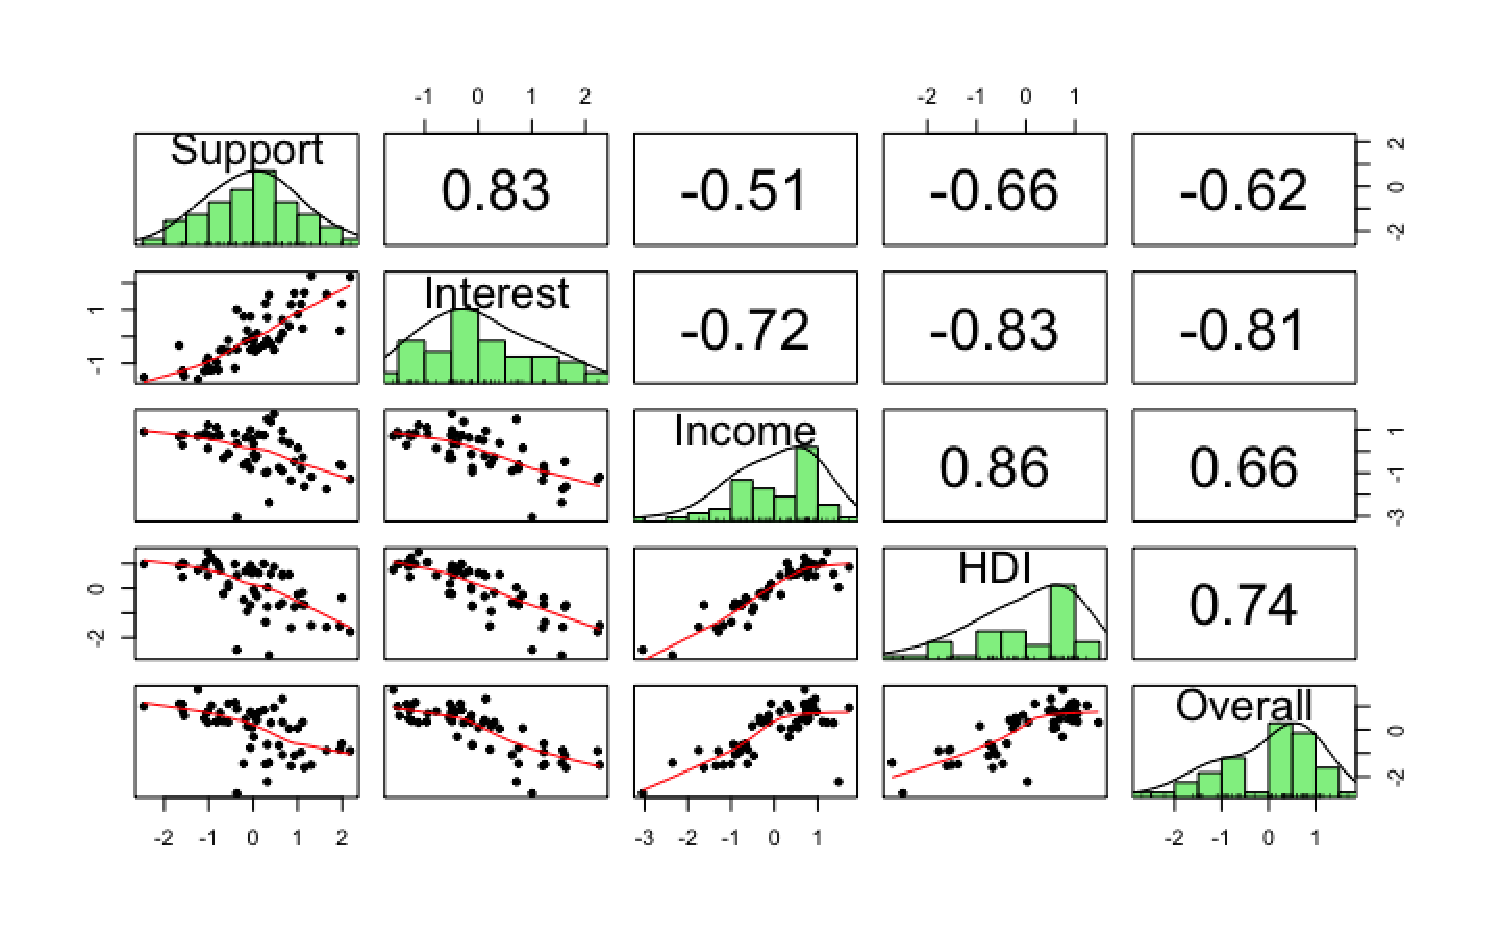
\includegraphics[width=\linewidth]{images/corr}
  \caption{Visualize Missing Data}
  \label{fig:corr}
\end{figure}


\subsection{regression Analysis}
\label{ss.reg}

\subsubsection{wealthier (higher income) countries and Support of Science}
\label{sss.incvssup}

To determine the relationship between a country's wealth (as indicated by its income) and the support it provides, we employed a linear regression analysis. The dependent variable in our model was "Support", and the independent variable was "Income". The model can be represented as:

$\text{Support} = -1.662 \times 10^{-16} - 0.4773 \times \text{Income} + \epsilon$

The model has an $R^2$ value of 0.2278, indicating that approximately 22.78\% of the variation in support can be explained by the country's income. The adjusted  $R^2$ is 0.213, which takes into account the number of predictors in the model and provides a more accurate representation of the model's explanatory power.

The results suggest that wealthier countries (with higher income) tend to provide less support. The negative coefficient for Income indicates that for every unit increase in income, the support decreases by 0.4773 units, on average, holding all else constant. The statistical significance of the coefficient (p-value < 0.05) provides evidence to reject the null hypothesis that income has no effect on support.


\subsubsection{Regression Analysis: Effect of HDI on Interest}
\label{sss.hdivsint}

To determine the relationship between a country's Human Development Index (HDI) and the level of interest (perhaps in a particular policy, investment, or other context). A simple linear regression model was used:

$\text{Interest} = -9.748 \times 10^{-16} - 0.8163 \times \text{HDI} + \epsilon$

The coefficient for HDI is -0.8163, which is statistically significant with a p-value much less than 0.05. This indicates that for every unit increase in HDI, the interest decreases by 0.8163 units, on average, holding all else constant. The strong negative relationship suggests that as countries have a higher Human Development Index, the level of interest tends to decrease.

The $R^2$  value of 0.6663 indicates that approximately 66.63\% of the variability in Interest can be explained by the HDI. The adjusted 
$R^2$  of 0.6599 provides a slightly more conservative estimate of the model's explanatory power, accounting for the number of predictors.

There is a significant negative relationship between a country's Human Development Index (HDI) and the level of interest. Specifically, as the HDI of a country increases, the level of interest tends to decrease. This model explains about 66.63\% of the variability in interest among the countries.


\subsubsection{Regression Analysis: Effect of Support and Interest on Overall}
\label{sss.supintvsoverall}

To determine the relationship between the level of "Support" and "Interest" a country receives or exhibits and an overall metric (which could be an overall satisfaction, rating, or any other measure).
A multiple linear regression model was employed:

$\text{Overall} = -1.445 \times 10^{-15} + 0.2502 \times \text{Support} - 0.9964 \times \text{Interest} + \epsilon$


The coefficient for Support is 0.2502. This indicates that for every unit increase in Support, the overall metric increases by 0.2502 units, on average, holding all else constant. However, the p-value for Support is 0.07782, which is slightly above the conventional 0.05 threshold for statistical significance. This suggests that the relationship between Support and Overall is suggestive but not strongly significant at the 5\% level.


The coefficient for Interest is -0.9964, which is statistically significant with a p-value much less than 0.05. This means that for every unit increase in Interest, the overall metric decreases by 0.9964 units, on average, holding all else constant. The strong negative relationship suggests that as Interest increases, the overall metric tends to decrease.

The $R^2$  value of 0.6537 indicates that approximately 65.37\% of the variability in the Overall metric can be explained by Support and Interest. The adjusted 
$R^2$ of 0.6402 provides a slightly more conservative estimate of the model's explanatory power, accounting for the number of predictors.

There is a suggestive positive relationship between Support and the Overall metric, though it's not strongly significant at the 5\% level. On the other hand, there is a significant negative relationship between Interest and the Overall metric. As Interest increases, the Overall metric tends to decrease. Together, Support and Interest explain about 65.37\% of the variability in the Overall metric among the countries.

\section{Key Findings}

%Results of the statistical analysis.
%Interpretation of these results in context.

In correlation and regression analysis, we found the variables which we are interested in are have linear relationship.
We can say, HDI has a negative effect on interest, Income has a negative effect to Support.
And Support have positive effect to Overall, but Interest has negative effect to it.

After we jump into country level analysis with standardlized all variables. 

Fig $\ref{fig:inc_sup}$ shows the Support do no have significance difference, which is approved the related model only have 22 precetage explliantion.
But, "Netherlands" have a abonormal Support score based on the income trend in countries level.


\begin{figure}[htb]
  \centering
  \includegraphics[width=\linewidth]{images/income_support_by_country}
  \caption{Income vs Support by Countries}
  \label{fig:inc_sup}
\end{figure}

% HDI $->$ Interest

Fig $\ref{fig:hdi_int}$ shows Lower HDI countries intend to have high interest in Science.
But, "United Kindom", and "Finland" are unique compare with the trend in countries level.

\begin{figure}[htb]
  \centering
  \includegraphics[width=\linewidth]{images/hdi_interest_by_country}
  \caption{HDI vs Interest by Countries}
  \label{fig:hdi_int}
\end{figure}

% Support, Interest -> Overall
Fig $\ref{fig:int_sup_overall}$ shows the lower Overall Score comes under area around 0.6 < Interest  < 0.7 and 0.4 < Support < 0.7.
And "Netherlands" and "Japan" shows unique pattern compare with the trend.

\begin{figure}[htb]
  \centering
  \includegraphics[width=\linewidth]{images/interest_support_vs_overall}
  \caption{Support vs Overall by Countries}
  \label{fig:int_sup_overall}
\end{figure}

\section{Recommendations and Future Research}

Based on the analysis and finding, 
The support of science in "Netherlands" in too low compare with similar income country.
May analysis work may be needed to figure the reason. we suggest their government may need to give more funding to support science related works.

"Finland" compare with other similar Human Development level countries shows science interest is too low.
We suggest give more investigation in anlaysis the reason of low interst in science for their students.

% \section{Limitations and Future Research}

% Limitations in data or methodology.
% Recommendations for future research.

\section{Conclusions}

% Final summary and conclusions drawn from the statistical analysis.
Many people assume that students from wealthy countries receive better support in science and are more interested in science. However, our research found that this is not the case. 
After analysis 54 countries data, we found low Human Development countries tend to higher interest in science.
It may be that the comfortable life of students in wealthy countries reduces their interest in scientific exploration.

Similar negative effect also comes from country Income to Support of science. But the difference between country not significant.

For individual country, Netherlands and Finland deserve special attention,
 the former show extremely support compare with other similar income countries
  and the latter's students shows lower interest in science compare with other similar Human Development countries.
% end of structure

\newpage
%
%\bibliographystyle{harvard}
\bibliographystyle{apalike3}
%\bibliographystyle{abbrv} %this is the same as plainnat but with last name fist 
%\bibliographystyle{unsrtnat}  % Sets the bibliography style
                              % unsrtnat. See the article about
                              % bibliography styles for more
                              % information on
                              % https://www.sharelatex.com/learn/Natbib_bibliography_styles
\bibliography{BIBTEX_GOF} 


\end{document}


